\clearpage
\section{Wertschöpfungskette}
\subsection{Modelle}
\subsubsection{Porter}
\begin{itemize}
	\item primär- \& sekundär(/support)-Aktivitäten
	\item erstere erreichen Wertschöpfung, letztere können das nicht (können erstere aber in ihrer Wertschöpfung unterstützen)
\end{itemize}
Dargestellt in Abbildung \ref{fig:porter_00} auf Seite \pageref{fig:porter_00}.
\begin{figure}[htb]
\centering
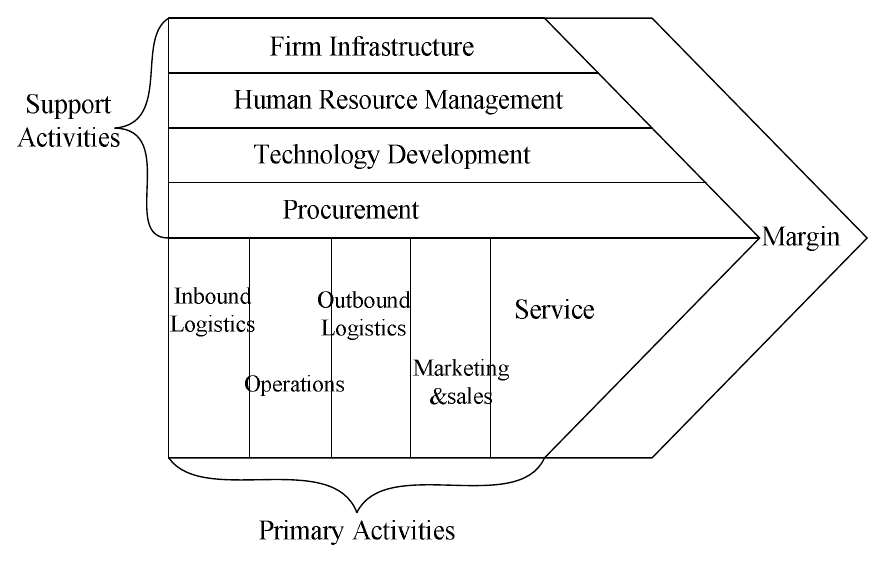
\includegraphics[width=\textwidth]{img/value_chain_porter.png}
\caption{Wertschöpfungskette nach Porter}
\label{fig:porter_00}
\end{figure}
\subsubsection{E-Commerce Wertschöpfungskette}
\begin{itemize}
	\item Primäraktivitäten 
	\begin{itemize}
		\item Information
		\item Bargaining
		\item Transaction
		\item Distribution
		\item Service
	\end{itemize}
	\item Operational Modes
	\begin{itemize}
		\item Organizational Model
		\item Operational Model
		\item Actual Support
	\end{itemize}
\end{itemize}
Dargestellt in Abbildung \ref{fig:ecvc_00} auf Seite \pageref{fig:ecvc_00}.
\begin{figure}[htb]
\centering
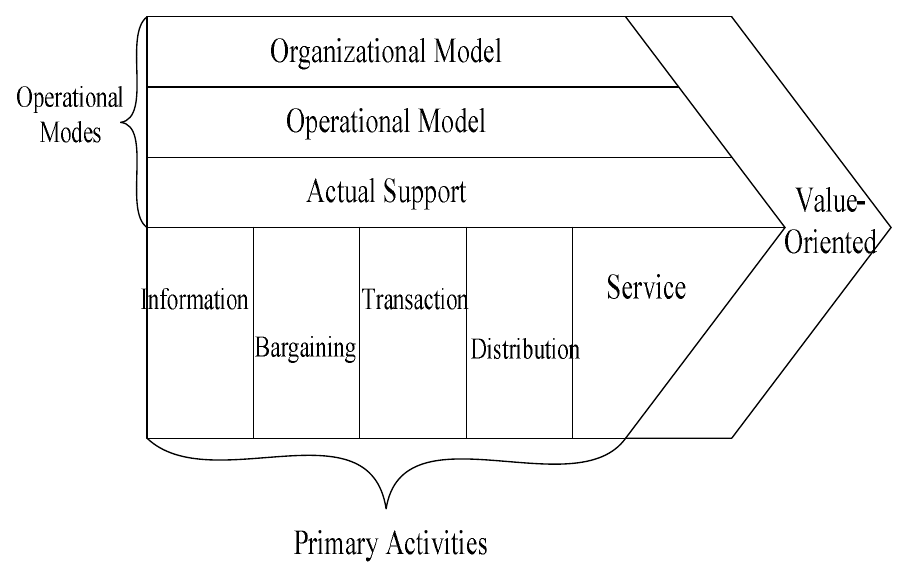
\includegraphics[width=\textwidth]{img/value_chain_ec1.png}
\caption{E-Commerce Wertschöpfungskette nach Mi Yan (Analysis on Mobile E-Commerce Value-Chain)}
\label{fig:ecvc_00}
\end{figure}
\subsubsection{Einordnung E-Payment in die EC Wertschöpfungskette}
Dargestellt in Abbildung \ref{fig:ecvc_01} auf Seite \pageref{fig:ecvc_01}.
\begin{figure}[htb]
\centering
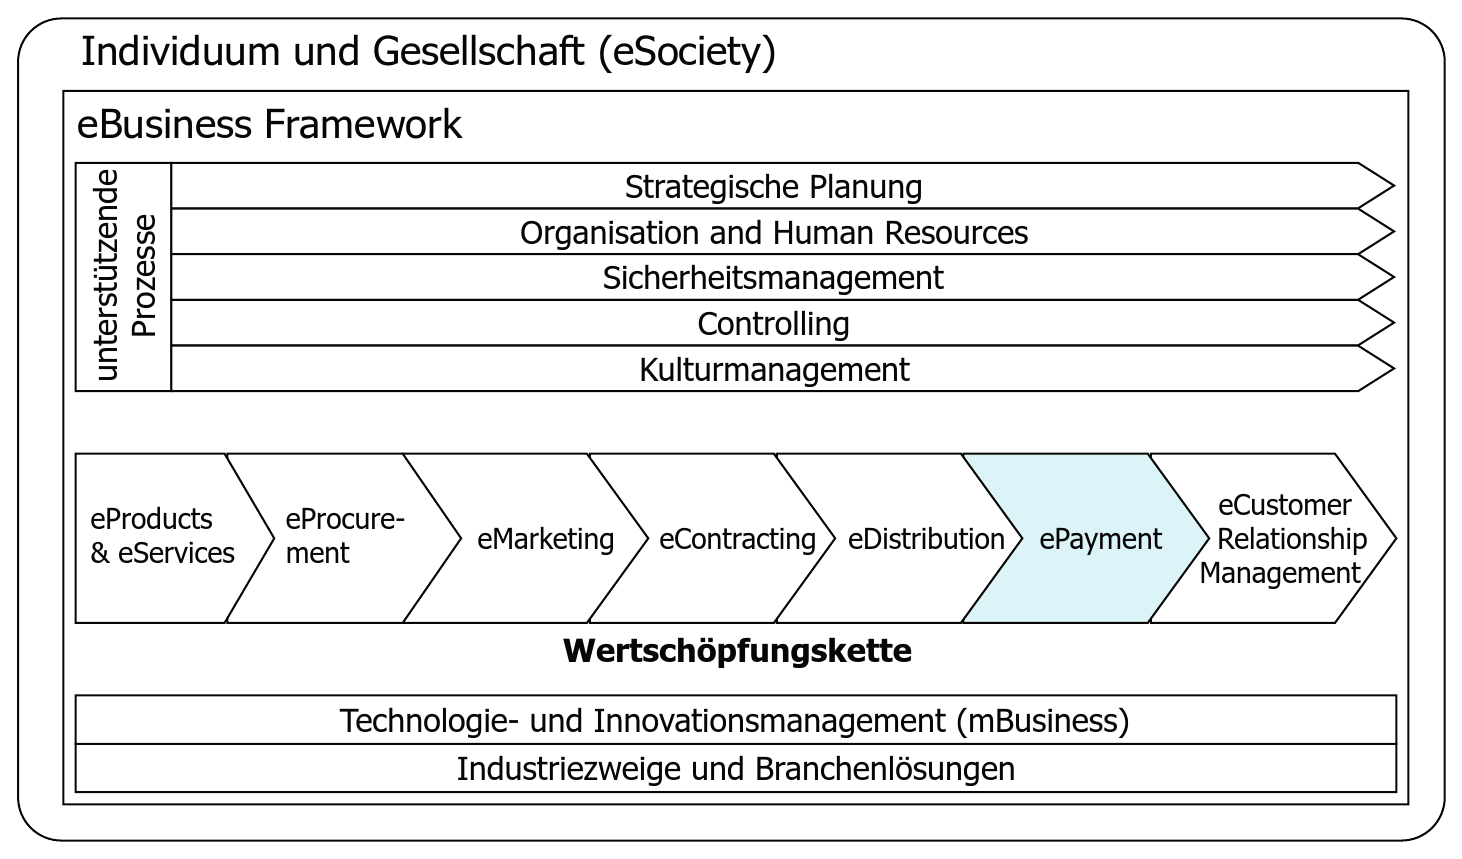
\includegraphics[width=\textwidth]{img/value_chain_ec2.png}
\caption{E-Commerce Wertschöpfungskette nach "eBusiness \& eCommerce - Management der digitalen Wertschöpfungskette"}
\label{fig:ecvc_01}
\end{figure}
\subsection{Analyse}
\textbf{Rayport und Sviokla}\\
Jede wertschöpfende Aktivität in der Wertschöpfungskette kann aufgeteilt werden in physische Wertschöpfung (basierend auf materiellen Resourcen, der traditionellen physischen Wertschöpfungskette) und Werschöpfung basierend auf Information als Rerource (virtuelle Wertschöpfungskette). In letztgenanner spielt Information nicht mehr nur eine unterstützende Rolle sondern aktive Komponente des Wertschöpfungsprozesses.\\
\\
"With the emergence of e-commerce, value prefers to establish on the infrastructure of data, information and knowledge."
